\documentclass[11pt]{amsart}
\usepackage[a4paper,margin=1in]{geometry}
\usepackage{amssymb}
\usepackage{tikz}
\usepackage{booktabs}
\usepackage[font=small,labelfont=bf]{caption}
\usepackage[hidelinks]{hyperref}

\colorlet{copper}{orange!75!black}
\colorlet{inkmuted}{black!60}
\tikzset{thin/.style={line width=0.4pt}}

\newtheorem{theorem}{Theorem}
\newtheorem{lemma}[theorem]{Lemma}
\theoremstyle{remark}
\newtheorem{remark}[theorem]{Remark}

\title{Incomplete Open Solids by Hand}
\author{Vamshi Jandhyala}
\address{London, United Kingdom}
\email{vamshi.jandhyala@gmail.com}

\begin{document}

\begin{abstract}
In 1974 Sol LeWitt exhibited the 122 incomplete open cubes: the connected sets of edges of a cube that are not contained in a plane and are not the whole cube, counted up to rotation. The count has been confirmed by careful checking and by computer, and the computer count has been extended to the other Platonic solids. We give a derivation of $122$ that can be checked with pencil and paper, and derivations of the same kind for the tetrahedron ($6$) and the octahedron ($185$), with the counts for each number of edges. Two ideas do the work. For many edges, Burnside's lemma counts all edge sets, and only a handful of them are disconnected. For few edges, one deletes the unused vertices and counts spanning trees of what is left, and those counts follow from one lemma about a cycle with a hub. The finite counts are checked in Lean.
\end{abstract}

\maketitle

\section{The question}

Take some of the twelve edges of a cube, built as a frame. LeWitt asked for the selections that are \emph{connected}, \emph{three-dimensional} (not lying in one plane) and \emph{incomplete} (not all twelve edges), and he counted two selections as the same when a rotation carries one to the other; mirror images count as different. He found $122$ of them and exhibited them all as sculptures and drawings~\cite{LeWitt}. Rozhkovskaya and Reb checked the list and found it complete, apart from one piece shown as a rotated copy where a reflection was intended~\cite{RR}; the counts by number of edges are in the OEIS~\cite{A393969}. Vejdemo-Johansson enumerated the analogous selections on all five Platonic solids by computer~\cite{VJ,A393693}.

In February 2026 Sam Hopkins asked on MathOverflow for a quick argument for $122$~\cite{MO}. The question had no answer when this note was written. This note gives one that fits on a few pages, and applies the same method to the tetrahedron and the octahedron. Before reading on, try the smallest case. A selection with three edges must use all three edge directions, so it is either a corner or a staircase. How many staircases are there up to rotation?

Call a set of edges of a polyhedron an \emph{incomplete open solid} if it is nonempty, connected, not contained in a plane, and not the whole edge set; write $a_k$ for the number of rotation classes with $k$ edges.

\begin{theorem}\label{thm:main}
The incomplete open tetrahedra, cubes and octahedra number $6$, $122$ and $185$, distributed by number of edges as in Table~\ref{tab:counts}.
\end{theorem}

\begin{table}[ht]
\centering
\begin{tabular}{l|rrrrrrrrr|r}
\toprule
$k$ & 3 & 4 & 5 & 6 & 7 & 8 & 9 & 10 & 11 & total\\
\midrule
tetrahedron & 3 & 2 & 1 & & & & & & & 6\\
cube & 3 & 5 & 14 & 24 & 32 & 25 & 13 & 5 & 1 & 122\\
octahedron & 5 & 16 & 34 & 46 & 38 & 27 & 13 & 5 & 1 & 185\\
\bottomrule
\end{tabular}
\caption{Rotation classes of incomplete open solids with $k$ edges.}
\label{tab:counts}
\end{table}

The totals are known~\cite{VJ}; what is new here is a derivation by hand, and, as far as we know, the octahedron row. The last three entries of the cube and octahedron rows agree, and Section~\ref{sec:remarks} explains why.

\section{Two tools}

\subsection{Many edges: Burnside and complements}

Let $G$ be the rotation group of the solid. Burnside's lemma~\cite[Ch.~6]{Aigner} says that the number of $G$-classes of $k$-edge sets is the average, over $g\in G$, of the number of $k$-edge sets that $g$ carries to themselves. A set is carried to itself exactly when it is a union of cycles of the permutation that $g$ induces on the edges, so if those cycles have lengths $\ell_1,\dots,\ell_r$, the number of fixed $k$-edge sets is the coefficient of $t^k$ in $\prod_i(1+t^{\ell_i})$. For example, a third-turn of the cube about a body diagonal moves the edges in four $3$-cycles, so the three-edge sets it fixes are the four single cycles, and indeed the coefficient of $t^3$ in $(1+t^3)^4$ is $4$.

The cube has $24$ rotations. The identity fixes every edge. The six quarter-turns about face axes move the edges in three $4$-cycles; the three half-turns about face axes, in six $2$-cycles; the six half-turns about axes through the midpoints of opposite edges fix those two edges and pair the other ten; and the eight third-turns about body diagonals move the edges in four $3$-cycles. Averaging,
\begin{equation}\label{eq:Z}
\begin{aligned}
Z(t)&=\tfrac1{24}\bigl[(1+t)^{12}+6(1+t^4)^3+3(1+t^2)^6+6(1+t)^2(1+t^2)^5+8(1+t^3)^4\bigr]\\
&=1+t+5t^2+13t^3+27t^4+38t^5+48t^6+38t^7+27t^8+13t^9+5t^{10}+t^{11}+t^{12}.
\end{aligned}
\end{equation}
The coefficient of $t^k$ counts all $k$-edge sets up to rotation, valid or not. The octahedron has the same polynomial: its twelve edges cross the cube's twelve edges at right angles in the dual position, and the rotations permute the two sets of edges in the same way. For many edges almost every set is valid, and it is enough to subtract the few disconnected ones.

\subsection{Few edges: delete the unused vertices}

A connected set with $k$ edges on $v$ vertices has $k\ge v-1$, with equality exactly for trees. When $k$ is small the set is usually a spanning tree of the vertices it uses, and it is easier to look at the vertices it does \emph{not} use. Fix the unused set $U$ up to rotation. The classes of trees whose unused set is a rotation of $U$ correspond to the classes of spanning trees of the graph on the other vertices under the stabiliser $H$ of $U$, the rotations that carry $U$ to itself. Burnside's lemma for $H$ counts these, so one needs the spanning trees and, for each $h\in H$, how many of them $h$ fixes. Most of the graphs that appear are a cycle with a hub, and their trees can be counted by which spokes they use.

Take a $4$-cycle with a hub joined to all four vertices, the wheel $W_4$ of Figure~\ref{fig:oct}(a). A spanning tree has four edges. With one spoke it must omit one of the four cycle edges, $4\cdot4=16$ trees. With two adjacent spokes, the cycle splits into arcs of lengths $1$ and $3$ between their ends; the tree must cut each arc once, since an uncut arc closes a cycle through the hub, so there are $1\cdot3$ ways for each of the four adjacent pairs, and $2\cdot2$ for each of the two opposite pairs. Three spokes leave arcs of lengths $1,1,2$, and four spokes leave four arcs of length $1$. In all,
\[
\underbrace{4\cdot4}_{s=1}+\underbrace{4\cdot(1\cdot3)+2\cdot(2\cdot2)}_{s=2}+\underbrace{4\cdot(1\cdot1\cdot2)}_{s=3}+\underbrace{1}_{s=4}=16+20+8+1=45,
\]
where $s$ is the number of spokes. The same reasoning works for any cycle with a hub.

\begin{lemma}\label{lem:hub}
Let $C$ be a cycle and join a new vertex, the hub, to some vertices of $C$ by spokes. Fix a nonempty set of $s$ spokes, and let $g_1,\dots,g_s$ be the lengths of the arcs of $C$ between consecutive attachment points of those spokes. The spanning trees that use exactly these spokes number $g_1g_2\cdots g_s$.
\end{lemma}

\begin{proof}
A spanning tree has one edge fewer than the number of vertices, so with $s$ spokes it omits exactly $s$ edges of $C$. If an arc lost no edge, the tree would contain that arc and the two spokes at its ends, a cycle. So each of the $s$ arcs loses at least one edge, and hence exactly one. Conversely, deleting one edge from each arc leaves $s$ paths, each attached to the hub by exactly one of the chosen spokes, which is a spanning tree. There are $g_i$ choices on the $i$-th arc.
\end{proof}

We also need the spanning trees of $K_4$: a tree on four vertices is a star (four of them, one for each centre) or a path ($4!/2=12$ of them), $16$ in all. Each tree has three of the six edges, so by symmetry each edge lies in $16\cdot3/6=8$ trees, and $K_4$ with one edge removed has $16-8=8$ spanning trees.

\section{The tetrahedron}

The rotations of a regular tetrahedron permute its four vertices by the twelve even permutations. Any three vertices are coplanar and the four are not, so a valid set is a connected set that uses all four vertices and is not all six edges: $k=3$, $4$ or $5$.

\emph{Three edges.} These are the $16$ spanning trees of $K_4$: four stars and twelve paths. The stars form one class. A path $a$--$b$--$c$--$d$ is fixed only by the identity and by its reversal $(a\,d)(b\,c)$, which is even; so each class of paths has $12/2=6$ members, and there are two classes, a path and its mirror image. Hence $a_3=3$.

\emph{Four edges.} The two missing edges are either disjoint, leaving a $4$-cycle, or share a vertex, leaving a triangle with a pendant edge. The three $4$-cycles are permuted transitively by the $3$-cycles. A triangle with a pendant edge is determined by the pendant vertex and its neighbour, an ordered pair; an even permutation fixing both must fix the other two vertices as well, so the twelve such sets form one class. Hence $a_4=2$, and $a_5=1$, for $3+2+1=6$.

\section{The cube}

A connected set lies in a plane exactly when it lies in a face, that is, when it uses at most two of the three edge directions. In particular every connected set with five or more edges is three-dimensional, since a face has four edges.

\subsection{Seven or more edges}

By~\eqref{eq:Z} there are $38,27,13,5,1$ classes of edge sets with $k=7,8,9,10,11$ edges. We subtract the disconnected ones, whose components each contain at least one edge. If $T$ is a set of vertices and $T'$ its complement, every edge not inside $T$ meets $T'$, and the edges meeting $T'$ number $3|T'|-e(T')$, where $e(\cdot)$ counts edges inside a vertex set. So
\[
e(T)=12-3|T'|+e(T').
\]
Two vertices span at most one edge, three at most two (the cube has no triangles), and four at most four (four vertices with five edges always contain a triangle). Hence six, five and four vertices span at most $7$, $5$ and $4$ edges, and two, three and four span at most $1$, $2$ and $4$. A disconnected set with three or more components therefore has at most $1+1+4=6$ edges. With two components on $p$ and $q$ vertices, $p+q\le8$, the largest totals are $1+7=8$ for $(2,6)$, $4+4=8$ for $(4,4)$ and $2+5=7$ for $(3,5)$; every other split gives at most $6$.

So no disconnected set has nine or more edges. With eight there are two classes: a lone edge with all seven edges on the remaining six vertices, and two opposite squares. With seven there are six:
\begin{itemize}
\item a lone edge with six of the seven edges on the other six vertices: the lone edge's stabiliser is the half-turn about the axis through its midpoint, which fixes just one of the seven edges (the opposite one) and pairs the rest, so there are $(7+1)/2=4$ classes;
\item a two-edge path with the five edges on the other five vertices: the path's three vertices must span two edges, and all two-edge paths are rotations of each other, so one class;
\item a square with three edges of the opposite square: one class.
\end{itemize}
Therefore $(a_7,a_8,a_9,a_{10},a_{11})=(38-6,\,27-2,\,13,\,5,\,1)=(32,25,13,5,1)$.

\begin{figure}[ht]
\centering
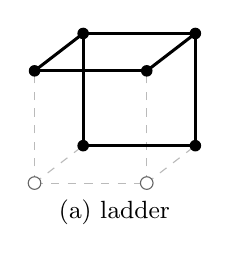
\begin{tikzpicture}[scale=0.95]
\draw[inkmuted!45,dashed,thin] (0.00,0.00)--(1.50,0.00);
\draw[inkmuted!45,dashed,thin] (0.00,0.00)--(0.65,0.50);
\draw[inkmuted!45,dashed,thin] (0.00,0.00)--(0.00,1.50);
\draw[inkmuted!45,dashed,thin] (1.50,0.00)--(2.15,0.50);
\draw[inkmuted!45,dashed,thin] (1.50,0.00)--(1.50,1.50);
\draw[line width=1.1pt,black] (0.65,0.50)--(2.15,0.50);
\draw[line width=1.1pt,black] (0.65,0.50)--(0.65,2.00);
\draw[line width=1.1pt,black] (2.15,0.50)--(2.15,2.00);
\draw[line width=1.1pt,black] (0.00,1.50)--(1.50,1.50);
\draw[line width=1.1pt,black] (0.00,1.50)--(0.65,2.00);
\draw[line width=1.1pt,black] (1.50,1.50)--(2.15,2.00);
\draw[line width=1.1pt,black] (0.65,2.00)--(2.15,2.00);
\draw[inkmuted,fill=white] (0.00,0.00) circle (2.4pt);
\draw[inkmuted,fill=white] (1.50,0.00) circle (2.4pt);
\fill[black] (0.65,0.50) circle (2.2pt);
\fill[black] (2.15,0.50) circle (2.2pt);
\fill[black] (0.00,1.50) circle (2.2pt);
\fill[black] (1.50,1.50) circle (2.2pt);
\fill[black] (0.65,2.00) circle (2.2pt);
\fill[black] (2.15,2.00) circle (2.2pt);
\node[below,font=\small] at (current bounding box.south) {(a) ladder};
\end{tikzpicture}
\hfill
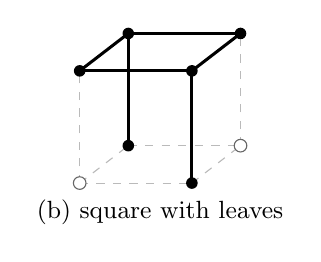
\begin{tikzpicture}[scale=0.95]
\draw[inkmuted!45,dashed,thin] (0.00,0.00)--(1.50,0.00);
\draw[inkmuted!45,dashed,thin] (0.00,0.00)--(0.65,0.50);
\draw[inkmuted!45,dashed,thin] (0.00,0.00)--(0.00,1.50);
\draw[inkmuted!45,dashed,thin] (1.50,0.00)--(2.15,0.50);
\draw[line width=1.1pt,black] (1.50,0.00)--(1.50,1.50);
\draw[inkmuted!45,dashed,thin] (0.65,0.50)--(2.15,0.50);
\draw[line width=1.1pt,black] (0.65,0.50)--(0.65,2.00);
\draw[inkmuted!45,dashed,thin] (2.15,0.50)--(2.15,2.00);
\draw[line width=1.1pt,black] (0.00,1.50)--(1.50,1.50);
\draw[line width=1.1pt,black] (0.00,1.50)--(0.65,2.00);
\draw[line width=1.1pt,black] (1.50,1.50)--(2.15,2.00);
\draw[line width=1.1pt,black] (0.65,2.00)--(2.15,2.00);
\draw[inkmuted,fill=white] (0.00,0.00) circle (2.4pt);
\fill[black] (1.50,0.00) circle (2.2pt);
\fill[black] (0.65,0.50) circle (2.2pt);
\draw[inkmuted,fill=white] (2.15,0.50) circle (2.4pt);
\fill[black] (0.00,1.50) circle (2.2pt);
\fill[black] (1.50,1.50) circle (2.2pt);
\fill[black] (0.65,2.00) circle (2.2pt);
\fill[black] (2.15,2.00) circle (2.2pt);
\node[below,font=\small] at (current bounding box.south) {(b) square with leaves};
\end{tikzpicture}
\hfill
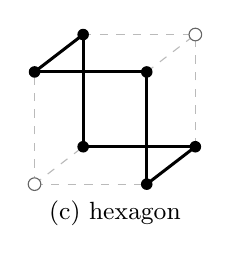
\begin{tikzpicture}[scale=0.95]
\draw[inkmuted!45,dashed,thin] (0.00,0.00)--(1.50,0.00);
\draw[inkmuted!45,dashed,thin] (0.00,0.00)--(0.65,0.50);
\draw[inkmuted!45,dashed,thin] (0.00,0.00)--(0.00,1.50);
\draw[line width=1.1pt,black] (1.50,0.00)--(2.15,0.50);
\draw[line width=1.1pt,black] (1.50,0.00)--(1.50,1.50);
\draw[line width=1.1pt,black] (0.65,0.50)--(2.15,0.50);
\draw[line width=1.1pt,black] (0.65,0.50)--(0.65,2.00);
\draw[inkmuted!45,dashed,thin] (2.15,0.50)--(2.15,2.00);
\draw[line width=1.1pt,black] (0.00,1.50)--(1.50,1.50);
\draw[line width=1.1pt,black] (0.00,1.50)--(0.65,2.00);
\draw[inkmuted!45,dashed,thin] (1.50,1.50)--(2.15,2.00);
\draw[inkmuted!45,dashed,thin] (0.65,2.00)--(2.15,2.00);
\draw[inkmuted,fill=white] (0.00,0.00) circle (2.4pt);
\fill[black] (1.50,0.00) circle (2.2pt);
\fill[black] (0.65,0.50) circle (2.2pt);
\fill[black] (2.15,0.50) circle (2.2pt);
\fill[black] (0.00,1.50) circle (2.2pt);
\fill[black] (1.50,1.50) circle (2.2pt);
\fill[black] (0.65,2.00) circle (2.2pt);
\draw[inkmuted,fill=white] (2.15,2.00) circle (2.4pt);
\node[below,font=\small] at (current bounding box.south) {(c) hexagon};
\end{tikzpicture}
\hfill
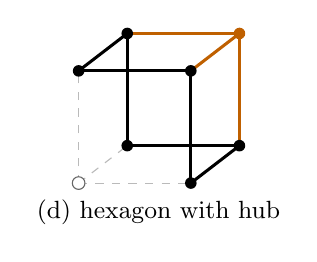
\begin{tikzpicture}[scale=0.95]
\draw[inkmuted!45,dashed,thin] (0.00,0.00)--(1.50,0.00);
\draw[inkmuted!45,dashed,thin] (0.00,0.00)--(0.65,0.50);
\draw[inkmuted!45,dashed,thin] (0.00,0.00)--(0.00,1.50);
\draw[line width=1.1pt,black] (1.50,0.00)--(2.15,0.50);
\draw[line width=1.1pt,black] (1.50,0.00)--(1.50,1.50);
\draw[line width=1.1pt,black] (0.65,0.50)--(2.15,0.50);
\draw[line width=1.1pt,black] (0.65,0.50)--(0.65,2.00);
\draw[line width=1.1pt,copper] (2.15,0.50)--(2.15,2.00);
\draw[line width=1.1pt,black] (0.00,1.50)--(1.50,1.50);
\draw[line width=1.1pt,black] (0.00,1.50)--(0.65,2.00);
\draw[line width=1.1pt,copper] (1.50,1.50)--(2.15,2.00);
\draw[line width=1.1pt,copper] (0.65,2.00)--(2.15,2.00);
\draw[inkmuted,fill=white] (0.00,0.00) circle (2.4pt);
\fill[black] (1.50,0.00) circle (2.2pt);
\fill[black] (0.65,0.50) circle (2.2pt);
\fill[black] (2.15,0.50) circle (2.2pt);
\fill[black] (0.00,1.50) circle (2.2pt);
\fill[black] (1.50,1.50) circle (2.2pt);
\fill[black] (0.65,2.00) circle (2.2pt);
\fill[copper] (2.15,2.00) circle (2.2pt);
\node[below,font=\small] at (current bounding box.south) {(d) hexagon with hub};
\end{tikzpicture}

\caption{The graphs left on the cube after deleting the unused vertices (hollow). (a)--(c): a pair at distance $1$, $2$, $3$, for five-edge trees. (d): one vertex, for six-edge trees; the hub and its three spokes are in copper.}
\label{fig:cube}
\end{figure}

\subsection{Five edges}

A connected five-edge set uses five or six vertices. On five vertices it contains a cycle, and the only cycles on at most five cube vertices are squares, so it is a square with a pendant edge: one class, since the four corners of a face are rotations of each other. On six vertices it is a tree, and the two unused vertices are at distance $1$, $2$ or $3$. Figure~\ref{fig:cube}(a)--(c) shows what remains.
\begin{itemize}
\item Distance $1$ leaves a ladder of two squares sharing a rung, with seven edges; a tree omits two of them. Of the $\binom72=21$ pairs, six disconnect the ladder (four isolate a corner and two cut off an end rung), so there are $15$ trees. The stabiliser is a half-turn that fixes the middle rung and pairs the other six edges; a fixed tree is the rung and two of the three pairs, $3$ trees. Classes: $(15+3)/2=9$.
\item Distance $2$ leaves a square with leaves at opposite corners: $4$ trees (delete one square edge). The stabiliser is a half-turn that moves every square edge, so $(4+0)/2=2$.
\item Distance $3$ leaves a hexagon: $6$ trees. The stabiliser has order $6$: two third-turns fix no edge, and three half-turns each fix two opposite hexagon edges, so each fixes $2$ trees. Classes: $(6+0+0+2+2+2)/6=2$.
\end{itemize}
Hence $a_5=9+2+2+1=14$.

\subsection{Six edges}

A connected six-edge set uses six or seven vertices (five vertices span at most five edges). On seven vertices it is a tree, and deleting the unused vertex leaves a hexagon and the opposite vertex as a hub joined to alternate hexagon vertices, Figure~\ref{fig:cube}(d). Lemma~\ref{lem:hub} gives, by the number of spokes,
\[
\underbrace{3\cdot6}_{\text{one}}+\underbrace{3\cdot(2\cdot4)}_{\text{two}}+\underbrace{2\cdot2\cdot2}_{\text{three}}=18+24+8=50
\]
trees. The stabiliser consists of the identity and two third-turns. A third-turn fixes a tree only if it keeps all three spokes and one of the two alternating triples of hexagon edges, so it fixes $2$ trees, and there are $(50+2+2)/3=18$ classes.

On six vertices the set has exactly one cycle, a square or a hexagon. Two hexagons: the unused pair is at distance $1$ or $3$ (distance $2$ leaves no hexagon). A square with two more edges: each corner of a square has one outward edge, so the extra edges are two leaves at adjacent or at opposite corners (two classes), or a two-edge tail at one corner. The tail turns left or right; these two are mirror images, and no rotation carries one to the other, since a rotation fixing a square and a corner is the identity. That makes six, and $a_6=18+6=24$.

\subsection{Three and four edges}

With at most four edges a cycle would be a square, which is flat, so the set is a tree using all three directions.

\emph{Three edges.} A corner (one class; $8$ corners, each fixed by its third-turns), or a staircase whose three steps go in three different directions. There are $24$ staircases: $12$ middle edges, and at each end of the middle edge one of the two other directions, chosen differently at the two ends. The half-turn about the axis through the midpoint of the middle edge swaps its ends and swaps the two other directions, so it fixes the staircase. Each staircase is therefore fixed by two rotations, its class has $12$ members, and there are two classes, a staircase and its mirror image. Hence $a_3=3$.

\emph{Four edges.} A branched tree has a vertex of degree three, with arms of lengths $2,1,1$: $8$ centres, and six ways to extend one of the three edges at the centre, so $48$ trees. A rotation fixing one must fix the centre and its long arm, and the third-turns at the centre move every arm, so only the identity fixes it: $48/24=2$ classes. A four-edge path uses one direction twice, never on consecutive steps. If the repeated steps are two apart (as in $xyxz$) there are $48$ such paths, and if they are three apart ($xyzx$) there are $24$; a rotation fixing a path fixes its middle vertex, and the third-turns there move the pair of path edges at that vertex, so again only the identity fixes a path. This gives $2+1=3$ classes of paths, and $a_4=2+3=5$.

Adding up, $3+5+14+24+32+25+13+5+1=122$.

\section{The octahedron}

Put the six vertices at $\pm e_1,\pm e_2,\pm e_3$. Two vertices are joined unless they are antipodal, so a vertex set $T$ spans
\[
e(T)=\tbinom{|T|}2-(\text{number of antipodal pairs in }T)
\]
edges. Three vertices span at most $3$ (a face), and four span $5$ if they contain one antipodal pair and $4$ if they contain two. Four vertices are coplanar exactly when they contain two antipodal pairs (an equatorial square). So a connected set is three-dimensional unless it uses at most three vertices or exactly the four vertices of an equator; in particular every set with five or more edges is three-dimensional.

\subsection{Five or more edges}

A disconnected set has components on at least two vertices each, with at most six vertices in all. Two components on $2+4$ vertices give at most $1+5=6$ edges, two on $3+3$ give at most $3+3=6$, and every other split gives at most $4$. So for $k\ge7$ every edge set is valid, and $a_7,\dots,a_{11}$ are the coefficients $38,27,13,5,1$ of~\eqref{eq:Z}.

For $k=6$ the disconnected sets are an edge with all five edges on the other four vertices (one class, since the rotations are transitive on edges), and two opposite faces (one class), Figure~\ref{fig:oct}(c),(d). So $a_6=48-2=46$.

For $k=5$ they are of two kinds. An edge with four of the five edges on the complementary four vertices: the stabiliser of the edge is a half-turn, which fixes one of those five edges and pairs the other four, giving $(5+1)/2=3$ classes. Two opposite faces with one edge removed: the six rotations preserving a pair of opposite faces act transitively on their six edges, giving one class. So $a_5=38-4=34$.

\begin{figure}[ht]
\centering
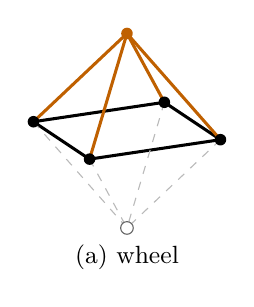
\begin{tikzpicture}[scale=0.95]
\draw[line width=1.1pt,black] (1.25,-0.12)--(0.50,0.38);
\draw[line width=1.1pt,black] (1.25,-0.12)--(-0.50,-0.38);
\draw[line width=1.1pt,copper] (1.25,-0.12)--(0.00,1.30);
\draw[inkmuted!45,dashed,thin] (1.25,-0.12)--(0.00,-1.30);
\draw[line width=1.1pt,black] (-1.25,0.12)--(0.50,0.38);
\draw[line width=1.1pt,black] (-1.25,0.12)--(-0.50,-0.38);
\draw[line width=1.1pt,copper] (-1.25,0.12)--(0.00,1.30);
\draw[inkmuted!45,dashed,thin] (-1.25,0.12)--(0.00,-1.30);
\draw[line width=1.1pt,copper] (0.50,0.38)--(0.00,1.30);
\draw[inkmuted!45,dashed,thin] (0.50,0.38)--(0.00,-1.30);
\draw[line width=1.1pt,copper] (-0.50,-0.38)--(0.00,1.30);
\draw[inkmuted!45,dashed,thin] (-0.50,-0.38)--(0.00,-1.30);
\fill[black] (1.25,-0.12) circle (2.2pt);
\fill[black] (-1.25,0.12) circle (2.2pt);
\fill[black] (0.50,0.38) circle (2.2pt);
\fill[black] (-0.50,-0.38) circle (2.2pt);
\fill[copper] (0.00,1.30) circle (2.2pt);
\draw[inkmuted,fill=white] (0.00,-1.30) circle (2.4pt);
\node[below,font=\small] at (current bounding box.south) {(a) wheel};
\end{tikzpicture}
\hfill
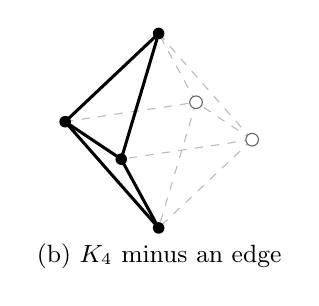
\begin{tikzpicture}[scale=0.95]
\draw[inkmuted!45,dashed,thin] (1.25,-0.12)--(0.50,0.38);
\draw[inkmuted!45,dashed,thin] (1.25,-0.12)--(-0.50,-0.38);
\draw[inkmuted!45,dashed,thin] (1.25,-0.12)--(0.00,1.30);
\draw[inkmuted!45,dashed,thin] (1.25,-0.12)--(0.00,-1.30);
\draw[inkmuted!45,dashed,thin] (-1.25,0.12)--(0.50,0.38);
\draw[line width=1.1pt,black] (-1.25,0.12)--(-0.50,-0.38);
\draw[line width=1.1pt,black] (-1.25,0.12)--(0.00,1.30);
\draw[line width=1.1pt,black] (-1.25,0.12)--(0.00,-1.30);
\draw[inkmuted!45,dashed,thin] (0.50,0.38)--(0.00,1.30);
\draw[inkmuted!45,dashed,thin] (0.50,0.38)--(0.00,-1.30);
\draw[line width=1.1pt,black] (-0.50,-0.38)--(0.00,1.30);
\draw[line width=1.1pt,black] (-0.50,-0.38)--(0.00,-1.30);
\draw[inkmuted,fill=white] (1.25,-0.12) circle (2.4pt);
\fill[black] (-1.25,0.12) circle (2.2pt);
\draw[inkmuted,fill=white] (0.50,0.38) circle (2.4pt);
\fill[black] (-0.50,-0.38) circle (2.2pt);
\fill[black] (0.00,1.30) circle (2.2pt);
\fill[black] (0.00,-1.30) circle (2.2pt);
\node[below,font=\small] at (current bounding box.south) {(b) $K_4$ minus an edge};
\end{tikzpicture}
\hfill
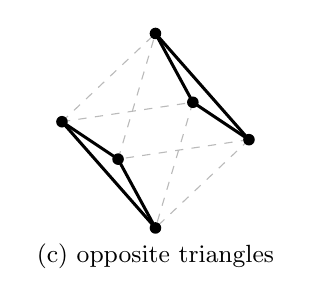
\begin{tikzpicture}[scale=0.95]
\draw[line width=1.1pt,black] (1.25,-0.12)--(0.50,0.38);
\draw[inkmuted!45,dashed,thin] (1.25,-0.12)--(-0.50,-0.38);
\draw[line width=1.1pt,black] (1.25,-0.12)--(0.00,1.30);
\draw[inkmuted!45,dashed,thin] (1.25,-0.12)--(0.00,-1.30);
\draw[inkmuted!45,dashed,thin] (-1.25,0.12)--(0.50,0.38);
\draw[line width=1.1pt,black] (-1.25,0.12)--(-0.50,-0.38);
\draw[inkmuted!45,dashed,thin] (-1.25,0.12)--(0.00,1.30);
\draw[line width=1.1pt,black] (-1.25,0.12)--(0.00,-1.30);
\draw[line width=1.1pt,black] (0.50,0.38)--(0.00,1.30);
\draw[inkmuted!45,dashed,thin] (0.50,0.38)--(0.00,-1.30);
\draw[inkmuted!45,dashed,thin] (-0.50,-0.38)--(0.00,1.30);
\draw[line width=1.1pt,black] (-0.50,-0.38)--(0.00,-1.30);
\fill[black] (1.25,-0.12) circle (2.2pt);
\fill[black] (-1.25,0.12) circle (2.2pt);
\fill[black] (0.50,0.38) circle (2.2pt);
\fill[black] (-0.50,-0.38) circle (2.2pt);
\fill[black] (0.00,1.30) circle (2.2pt);
\fill[black] (0.00,-1.30) circle (2.2pt);
\node[below,font=\small] at (current bounding box.south) {(c) opposite triangles};
\end{tikzpicture}
\hfill
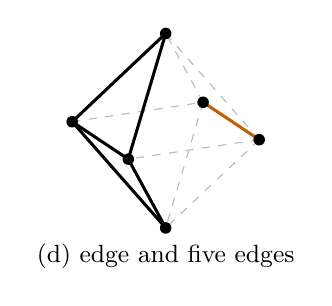
\begin{tikzpicture}[scale=0.95]
\draw[line width=1.1pt,copper] (1.25,-0.12)--(0.50,0.38);
\draw[inkmuted!45,dashed,thin] (1.25,-0.12)--(-0.50,-0.38);
\draw[inkmuted!45,dashed,thin] (1.25,-0.12)--(0.00,1.30);
\draw[inkmuted!45,dashed,thin] (1.25,-0.12)--(0.00,-1.30);
\draw[inkmuted!45,dashed,thin] (-1.25,0.12)--(0.50,0.38);
\draw[line width=1.1pt,black] (-1.25,0.12)--(-0.50,-0.38);
\draw[line width=1.1pt,black] (-1.25,0.12)--(0.00,1.30);
\draw[line width=1.1pt,black] (-1.25,0.12)--(0.00,-1.30);
\draw[inkmuted!45,dashed,thin] (0.50,0.38)--(0.00,1.30);
\draw[inkmuted!45,dashed,thin] (0.50,0.38)--(0.00,-1.30);
\draw[line width=1.1pt,black] (-0.50,-0.38)--(0.00,1.30);
\draw[line width=1.1pt,black] (-0.50,-0.38)--(0.00,-1.30);
\fill[black] (1.25,-0.12) circle (2.2pt);
\fill[black] (-1.25,0.12) circle (2.2pt);
\fill[black] (0.50,0.38) circle (2.2pt);
\fill[black] (-0.50,-0.38) circle (2.2pt);
\fill[black] (0.00,1.30) circle (2.2pt);
\fill[black] (0.00,-1.30) circle (2.2pt);
\node[below,font=\small] at (current bounding box.south) {(d) edge and five edges};
\end{tikzpicture}

\caption{The octahedron. (a) One unused vertex leaves the wheel $W_4$; the hub and spokes are in copper. (b) An unused edge leaves $K_4$ minus an edge. (c), (d) The two disconnected six-edge sets.}
\label{fig:oct}
\end{figure}

\subsection{Four edges}

On four vertices a four-edge set contains a cycle, and the vertices must not form an equator, so they contain one antipodal pair $\{a,b\}$ and span the five edges of $K_4$ minus the edge $ab$. Removing the edge $cd$ joining the other two leaves a skew $4$-cycle; removing one of $ac,ad,bc,bd$ leaves a triangle with a pendant edge. Such vertex sets are the complements of the edges, so they form one class, and the stabiliser swaps $a\leftrightarrow b$ and $c\leftrightarrow d$, pairing $ac$ with $bd$ and $ad$ with $bc$. That gives $1+2=3$ classes.

On five vertices the set is a spanning tree, and deleting the unused vertex leaves the wheel $W_4$, Figure~\ref{fig:oct}(a), with $45$ spanning trees by Lemma~\ref{lem:hub}. The stabiliser is the four rotations about the axis through the unused vertex. A quarter-turn fixes only the star of all four spokes. The half-turn fixes the star and the four trees made of two opposite spokes and two opposite square edges. Classes: $(45+1+1+5)/4=13$. Hence $a_4=3+13=16$.

\subsection{Three edges}

Three edges on three vertices form a face, which is flat. Otherwise the set is a tree on four vertices that are not an equator, so it is one of the $8$ spanning trees of $K_4$ minus an edge, Figure~\ref{fig:oct}(b). With the labels above, the half-turn of the stabiliser fixes the two trees $cd,ac,bd$ and $cd,ad,bc$, so there are $(8+2)/2=5$ classes. Fewer edges use at most three vertices. Hence $a_3=5$, and the total is $5+16+34+46+38+27+13+5+1=185$.

\section{Remarks}\label{sec:remarks}

The cube and the octahedron share the polynomial~\eqref{eq:Z}, so their counts can differ only through invalid sets. On the cube every set with at least nine edges is valid, and on the octahedron every set with at least seven, which is why the last three entries of Table~\ref{tab:counts} agree. The octahedron's extra classes all have at most six edges, where its graph, with triangles and vertices of degree four, allows more connected shapes than the cube's.

We have not tried the dodecahedron and icosahedron, which have $30$ edges and millions of classes~\cite{VJ}. There the middle range of edge counts, where neither disconnected sets nor spanning trees are scarce, is too wide for either tool.

\section{Verification}

The finite numbers above are checked in Lean~4 with Mathlib~\cite{mathlib}: the $24$ rotations and their cycle types on the edges of both solids, the polynomial identity~\eqref{eq:Z}, the bounds on edges spanned by few vertices, every spanning-tree count (by number of spokes where the text counts that way), the number of trees fixed by each element of each stabiliser, and the final sums. The graphs are built from the solids by deleting vertices, not typed in, and the small checks are done by kernel reduction. Burnside's lemma and the case analyses are in the text and not formalised. Two Python scripts check every intermediate count of the text exhaustively, including the classification of disconnected sets and the shapes in each case, and an independent script enumerates all edge sets of both solids directly. The two audit scripts and the Lean files are mutation-tested: deliberately wrong variants (identifying mirror images, keeping flat sets, a wrong tree count, a wrong fixed-point count) must fail. Code and Lean files are at~\cite{repo}.

\section*{Acknowledgments}

The question is due to Sam Hopkins. The cube argument was first developed with OpenAI Codex; the tetrahedron and octahedron counts, the computations and the Lean formalisation were carried out with Claude Opus~5.5 (Anthropic). A comment under the question links a shared ChatGPT conversation that the author could not open, so any overlap with it is unknown. The author is responsible for the content.

\begin{thebibliography}{9}
\bibitem{Aigner} M.~Aigner, \emph{A Course in Enumeration}, Graduate Texts in Mathematics 238, Springer, Berlin, 2007.
\bibitem{LeWitt} S.~LeWitt, \emph{Incomplete Open Cubes}, John Weber Gallery, New York, 1974.
\bibitem{MO} S.~Hopkins, \emph{Quick argument for Sol LeWitt's count of 122 incomplete open cubes}, MathOverflow question 508521 (2026), \url{https://mathoverflow.net/q/508521}.
\bibitem{A393969} OEIS Foundation, \emph{The On-Line Encyclopedia of Integer Sequences}, sequence A393969 (P.~Xausa), \url{https://oeis.org/A393969}.
\bibitem{A393693} OEIS Foundation, \emph{The On-Line Encyclopedia of Integer Sequences}, sequence A393693 (M.~Marcus), \url{https://oeis.org/A393693}.
\bibitem{RR} N.~Rozhkovskaya and M.~Reb, \emph{Is the list of incomplete open cubes complete?}, Nexus Netw. J. 17 (2015), 913--925.
\bibitem{VJ} M.~Vejdemo-Johansson, \emph{Incomplete open Platonic solids}, arXiv:2602.20425 (2026).
\bibitem{mathlib} The mathlib Community, \emph{The Lean mathematical library}, in: Proc. 9th ACM SIGPLAN Int. Conf. on Certified Programs and Proofs (CPP 2020), 367--381.
\bibitem{repo} V.~Jandhyala, code and Lean proofs, \url{https://github.com/jvvk/mathematics/tree/main/incomplete-open-solids}.
\end{thebibliography}

\end{document}
